\documentclass[12pt]{article}
\pagenumbering{arabic}
\pdfpagewidth 8.5in
\pdfpageheight 11in
\setlength\topmargin{0in}
\setlength\headheight{0in}
\setlength\headsep{0in}
\setlength\textheight{9.0in}
\setlength\textwidth{6.5in}
\setlength\oddsidemargin{0in}
\setlength\evensidemargin{0in}
\setlength\parindent{0.25in}
\setlength\parskip{0.25in}
\parskip 0.0pt
\usepackage[utf8]{inputenc}
\usepackage[english]{babel}
\usepackage{amsmath}
\usepackage{amsfonts}
\usepackage{amssymb}
\usepackage{amsbsy}
\usepackage{setspace}
\usepackage{graphicx}
\usepackage{tabularx,ragged2e,booktabs,caption}
\usepackage{float}
\usepackage{dcolumn}
\usepackage{natbib}
%\usepackage{biblatex}
\usepackage{subfigure}
\usepackage{hyperref}
%\usepackage{authblk}
\usepackage{footmisc}

\makeatletter
\makeatletter
\renewcommand*{\@fnsymbol}[1]{\ifcase#1\or*\or a\or b\else\@arabic{#1}\fi}
\makeatother
\makeatother

\begin{document}  


\begin{titlepage}




%	\begin{center}

\title{A Dynamic Model of Dissent and Political Stability \thanks{Conflicts of interest: none. This research did not receive any specific grant from funding agencies in the public, commercial, or not-for-profit sectors.}}

\author{Ethan Spangler\thanks{Corresponding Author. Email: {\href{mailto:eospangler@gmail.com}{eospangler@gmail.com}}; Tel: 801-458-9923}\\%; Washington State University School of Economic Sciences Hulbert Hall 101, Pullman, WA 99164, United States}  \\
Ben Smith\thanks{Email: {\href{mailto:bosmith@unomaha.edu}{bosmith@unomaha.edu}}; University of Nebraska-Omaha Mammel Hall, Suite 332, 6708 Pine Street, Omaha, NE 68182, United States}}

%\vfill

% Bottom of the page
\date{\today}
%\end{center}
\maketitle


\begin{abstract}
\noindent The importance of political stability is well established and can affect all aspects of an economy. However, despite its significance, theoretical models of political stability remain underdeveloped. As demonstrated by the recent uprisings in the Middle East and populist fervor in the US and Europe, current models inadequately explain either. Our model extends the work of previous scholars by focusing on the interactions of a non-altruistic government and its citizenry. The government maximizes its own stability by choosing its level of public and security allocations, subject to a resource constraint and the level of discontent from the citizenry. In turn, each member of the public chooses their level of dissent, based on their own preferences and the risk of punishment. Through simulation we show how exogenous shocks at the government and individual levels can affect political stability. The end goal is a model that can help provide new insights into evaluating a country's political stability. Our findings suggest that countries can be stable in their political instability and that counties with a preference for using government services over suppression are more likely to be politically stable.      


\end{abstract}

\noindent \textit{Keywords}: Political Stability, Dissent, Simulation \\

\noindent \textit{JEL Code}: H1, C15, P16


\end{titlepage}

\begin{spacing}{1.5}


\section{Introduction}

The past decade has seen dramatic political shifts in both the developing and developed worlds. In December 2010 mass protests and demonstrations erupted across Tunisia, demanding an end to the autocratic regime of Ben-Ali. For years Tunisia had been plagued by corruption, high unemployment, inflation, and many other systemic problems that the government failed to address. The Tunisian protests quickly turned into a full scale revolution and Ben-Ali was forced to flee the country a mere two months after protests began. Spurred by the success in Tunisia and facing the same governmental failures, long suppressed public outrage unleashed itself and cascaded through the rest of North Africa and the Middle East, resulting in what is now referred to as the Arab Spring. While the events of the Arab Spring are still unfolding, thus far it has resulted in complete regime changes in Tunisia, Libya, and Egypt, ongoing civil wars in Syria and Yemen, and political concessions in many other countries (The Economist, 2016).  

While less explosive, the developed world has seen its own manifestations of political instability. A UK referendum rejected continued membership in the EU, a move that surprised much of the world. In the US, Donald Trump, a man that has never held public office, rode a wave of populist rhetoric into the White House; beating a candidate considered to be a political insider. Other Western countries have seen formerly fringe parties either be elected into office or make substantial legislative gains. In each case, populist policies and politicians were carried into office in part by a public that felt the previous governments had failed to address their concerns adequately (Judis, 2016).

Surface analysis of the Arab Spring and Western populism may find few parallels between them, but at a deeper level the two are quite similar. In both cases, the governments of each failed to address the concerns of large sections of the public. The only difference between the two is that with the Arab Spring, there were no nonviolent means to enact change to the government whereas in the West there are non-violent means to change the government, i.e. voting. While the means may have differed, riots vs. ballots, the effect was often the same, a change in government. Part of why these events were so surprising may be the under development of models connecting public dissent and a country's political stability. A better understanding of political stability is important because it can significantly impact economic growth (Alesina and Perotti, 1996; Jong-A-Pin, 2009; Aisen and Veiga, 2013). 

%The role of dissent 

%on how the interactions of a government and its citizens affects a country's political stability. 

%Part of why these events were so surprising may be the lack of a model on how the interactions of a government and its citizens affects a country's political stability. It is common in economics to view the government as a benevolent social planner, a fictitious but theoretically convenient entity, seeking to maximize social welfare. Some theoretical developments have stepped away from absolute benevolence and introduce a measure of corruption (Acemoglu and Robinson, 2001), but the overall set up remains. A better understanding of political stability is important because it can significantly impact economic growth (Alesina and Perotti, 1996; Jong-A-Pin, 2009; Aisen and Veiga, 2013).

This paper develops a theoretical model concerning the dynamic interactions between a non-altruistic government and its public and how that relationship affects political stability. This paper constructs a model of governance robust enough to account for both authoritarian and democratic countries. Using simulations we are able to show that countries can display a consistent pattern of political instability but not succumb to governmental failure. Additionally, we find that governments that favor soft power tend to be more stable, regardless of total government resources. Overall we feel this model can provide basis for new studies of political stability.  
  
The structure of this paper is as follows: a review of the literature concerning political stability, our theory on the structure of dissent and political stability, simulations and analysis, and finally conclusion.    

\section{Related Literature}

%Expand and work in Epstein (2002) ABM paper civil violence 

The bulk of the literature concerning political stability focuses on the factors motivating revolt and revolution. Grossman (1991), Acemoglu and Robinson (2001), MacCulloch (2001 and 2005), Apolte (2012a) explore the role of income inequality in fomenting revolution. Other approaches concentrate on the role of regime types (Guttman and Reuveny, 2014) or government institutions (Goldstone et al., 2010; Acemoglu et al, 2012; Fukuyama 2014). The general findings of these works is that the more unequal a society is and the less effective its institutions, the more unstable the country will likely be. 

%Another body of literature has been focusing on what type of governement emerges after a transition (Acemoglu and Robinson, 2008; Acemoglu et al. 2010)

%They're all making the same binary choice. Rebel or not. 

Diverging from the top down macroeconomic approach, literature from the public choice field applies an individual approach. Tullock's (1971 and 1974) seminal works concerning the economics of rebellion focus on the paradoxical observation that while it seems inherently irrational for an individual to join a rebellion, objective evidence is to the contrary since revolutions have occurred and will continue to. In essence, the problem is how do people cooperate enough to form a functional rebellion. 

Tullock answers this problem by focusing on the potential material gains that could come from a successful rebellion (1971 and 1974). Kurrild-Klitgaard (1997), Bueno de Mesquita (2010), and Apolte (2012a and 2012b) all build from the foundation by Tullock and offer their own solutions to the `paradox of rebellion' but remain within the game theoretic structure. A central element of these models is the individual making a binary choice of whether to rebel or not. 
 
Clearly an important factor in the decision to rebel are the potential gains one might achieve but another critical component are the other participating members. The distinction between a few dissidents being rounded up by police and the complete upheaval of the political order is one of numbers. The concept of social `critical mass' or `tipping point' is discussed by Schelling (1978) and Gladwell (2000) and more formally modeled by Granovetter (1978). The idea is that an individual's decision to join a social movement, like a rebellion, is dependent on their own preferences for rebellion and how many individuals are already engaged in the movement. Kuran (1989) goes further, modeling the individual choice but extending it to show that there are thresholds with respect to political stability. Once these threshold are breached, a revolution can materialize unexpectedly. However, the individual is still making a binary choice of whether to rebel or not. 

%Rebellion is a level in our model! Not a binary choice!
%Clean this up  

The model presented in this paper diverges from the literature in two important ways. First, we view dissent as a level not binary. When a individual chooses to rebel against their government, it is not a simple dichotomist choice. Writing a strongly worded letter is not the same as storming the gates of the castle. When dissenting, individuals choose what their level of dissent will be. By treating dissent as a level variable, it gives this model a high degree of nuance and to the best of the authors' knowledge is the first to do so. Another advantage of treating dissent as a level is that it allows this model to be used in situations where a small but vocal minority is able to affect political stability. 

Second, the authors of this paper believe that the focus on revolution, though valuable, does not capture the entirety of the situation. Revolution is the end point of a long process. A nation can exist for a long time in a state of low political stability but not descend into revolt; i.e. be stable in its instability. Instead this model focusing on the decisions and dynamics that precipitate a revolution. By focusing on the dynamics preceding a revolution, we avoid the theoretical difficulties of the collective action problem explored by the paradox of rebellion literature.  

The model presented here has its roots in Buchanan and Tullock (1962) but extends it to incorporate Acemoglu and Robinson's (2001) self interested government and Kuran's (1989) threshold. Our focus is on the dynamic interactions of a non-altruistic government and its citizenry. This paper bridges the institutional and public choice approaches to include both the effectiveness of government institutions and an individual's choice to dissent. The goal of this paper is not to predict the spark that ignites a revolution, but instead to examine the environment that allows a spark to turn into a revolution. Through simulation we explore how countries with differing parameter values react and handle various exogenous shocks. 

%OUr parameters settings reflect institutional differences! Say that! 

\section{Theory}

%define political stability and individual dissent 
Before delving into the the model, it is important to establish our working definition of `political stability'. For the purposes of this paper, political stability, $\Lambda_t$, is defined as the ability of a government to survive an exogenous shock at time $t$. This makes $\Lambda_t$ a measure of governmental resiliency at a given point in time. Political stability is related to but different than political risk. Political risk is when a government negatively interferences with business operations (Kobrin, 1979). Political stability is related to how much control the government has. So long as $\Lambda_t>0$ the government continues to function. However, as $\Lambda_t\rightarrow 0$ the government's position becomes more precarious. Should $\Lambda_t \leq 0$ for a sustained period, then the government has failed.  

\begin{figure}[htb]
\centering 
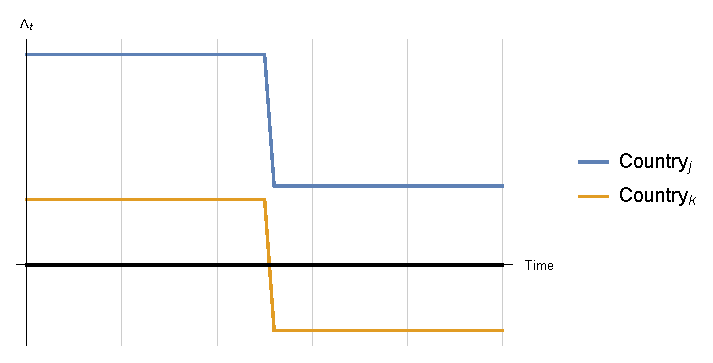
\includegraphics
[width=0.45\textwidth]{Mutual_shock.eps} 
\caption{Country Resiliency}
\end{figure}

This notion of governmental resiliency is illustrated in Figure 1. Here we have two countries of differing levels of $\Lambda_t$, Country$_j$ and Country$_k$. Both countries experience a shock that decreases each's political stability by the same magnitude. Because Country$_j$ was previously at a higher level of political stability than Country$_k$, the government of Country$_j$ survives while Country$_k$'s does not. Our definition of political stability is less rigid than previous methods, allowing political stability to fluctuate realistically. In developing this theoretical model we felt it was important to ground it in a narrative that closely adhered to reality.      


%It also allows a country to experience temporary crisis,$\Lambda_{t^*}$, without it fully failing. Figure 2 shows these situations graphically.
%\begin{figure}[htb]
%\centering 
%\subfigure{\includegraphics
%[width=0.45\textwidth]{Stable_Instability.eps}} 
%\subfigure{\includegraphics
%[width=0.45\textwidth]{Temporary_Crisis.eps}} 
%\caption{$\Phi$ Shock}
%\end{figure}







\subsection{Model}

%Discuss why a functional form.


`In perpetrating a revolution, there are two requirements: someone or something to revolt against and someone to actually show up and do the revolting.' (Allen, 1975 p. 107). In this paper we adopt a same mentality as Allen by incorporating the actions of both the government and the people. The model begins in period 0, the catalyst being the initial amount of total dissent, $D_0$. This $D_0$ can be thought of as either anarchists or remnants of the previous regime. 

The notion that some subsection of the population will always be dissatisfied with the government is in line with the `median voter theorem' (Congleton, 2003) wherein any policy choice inevitably displease some portion of society. A government then forms to manage and organize affairs, setting initial policy choices. The government maximizes political stability by choosing its level of civil and security allocations, subject to a budget constraint and the level of discontent from the citizenry. In turn, each member of the public chooses their level of dissent based on their own constraints and preferences as well as the probability of punishment. This dynamic interaction repeats until state failure ($\Lambda_t\leq 0$). 

%Why did I do everything in an explicit functional form? Because I needed a functional form to do the simulations, so might as well same time and do that from the start.  
 
\subsection{Individual's Problem}

Initial framing of the individual's problem begins in the general sense as a household problem, 

\begin{equation}
	U(c,l) \text{ s.t. } M %& E 
\end{equation}

\noindent where utility, $U(c,l)$, is a function of consumption, $c$ and leisure, $l$, subject to an income, $M$,  constraint. This represents the aspects of an individual's life that they have control over. However, there are some things an individual cannot control.  

In daily life, individuals face societal problems. It could be as mundane as a long line at the DMV\footnote{In the US the Department of Motor Vehicles (DMV) is a notoriously inefficient government office in the US.}. Perhaps they encountered a corrupt police officer. Another scenario could involve members of a different group harassing the individual. Maybe they saw a story about a wealthy, well-connected elite dodging criminal charges. Whatever the particular issue, it is a problem that the individual cannot solve themselves, but it has negatively affected their life. These are societal issues that only a government could properly address. However, the government is unable and/or unwilling to address these problems completely to the satisfaction of the individual. Without any direct power to alter their situation the individual does what people usually do in such situations, they dissent. 

Our origin for dissent is very similar to Gurr's (2015) concept of `relative deprivation' wherein the perceived difference between a person's value expectation and their value capabilities insights political action. However, here we are emphasizing the relationship between the individual and their government. The incongruity between an individual's expectations of what a government should do and the reality of what a government does do results in dissent.

Having already solved their household problem, the individual then uses a portion of what would be their leisure and instead uses it to dissent, which provides a cathartic release. Dissenting gives the individual some level of utility, with how much extra utility dictated by individual preferences and external parameters. Tullock (1971 and 1974) focuses primarily on the material gains from revolt, but also suggests that there could be potential non-material benefits of rebellion for the individual. However, Tullock views these non-material benefits more as possible entertainment whereas we view dissent as therapeutic, a subtle but nuanced difference. 

The individual maximizes utility from dissenting based on costs and benefits. Additionally, because the individual is using resources that would otherwise be used for leisure, this places an upper limit on the amount of dissent any individual can do. 

\vspace{.5 em}
\noindent Individual's Problem:
\begin{equation}
{\underset{d_{i,t}}{\text{max }}}  U_{i,t}= \frac{{d_{i,t}}^{{x}_i}}{g_t  E} - P_t \left( \bar{d}_{t-1} \Bigg|\frac{D_{t-1}}{S_t},\sigma \right)d_{i,t}^A
\end{equation}

\noindent where:
\begin{itemize}
	\item $d_{i,t}$ is individual dissent.  
	\item ${x}_i$ is the individual's activism preference. 
	\item $g_t$ is benefit from the government. 
	\item $E$ is the individual environment/quality of life. 
	\item $P_t \left( \bar{d}_{t-1} \Bigg|\frac{D_{t-1}}{S_t},\sigma \right)$ is the probability of being caught dissenting. 
	\item $\bar{d}_{t-1}$ is average individual dissent from the previous period.  
	\item $D_{t-1}$ total dissent from the previous period.
	\item $S_t$ is government security goods and services. 
	\item $\sigma$ is government policing efficiency. 
	\item $A$ is the punishment parameter. 
\end{itemize}
 
$ d_{i,t} $ is the amount individual $i$ dissents in period $t$ and is treated as a level variable wherein each period an individual chooses their level of dissent based on the situation they find themselves in and their own preferences. We assume dissent takes only non-negative values, $d_{i,t}\geq0$. Different levels of $d_{i,t}$ have different interpretations. An individual with $d_{i,t}=0$ is interpreted as not dissenting, this person is either content with the government or too scared to dissent. Alternatively a positive value of $d_{i,t}$ can be interpreted as being more active. On the low end, $d_{i,t}>0$, could be contacting government representatives, attending open forums, voting for opposition parties, or kvetching about politics with colleagues. At the extreme end, $d_{i,t}>>0$, dissent takes on a more active or revolutionary bent: protests, riots, molotovs. Since individuals dissent during time they would otherwise be using for leisure there is a maximum amount a single individual can dissent for a given period, ${d_{i,t}}^{max}$. 

$x_i$ is the exponent that represents an individual's activism preference with respect to dissenting. We assume $x_i \sim logN(0,1)$, the Log-Normal PDF. Different values of $x_i$ have different interpretations. As show in Figure 2, an individual with a $x_i$ on the left of the distribution (the darker shades) could be seen an individual with high anxiety when it comes to dissenting. However, as we move to the right of the distribution (lighter shades), the individual becomes more amenable to dissent. Near the peak, these individuals might be comfortable discussing their frustrations among close peers (`dinner party dissenters') but more active actions is unlikely. As we move to the far right, each higher value of $x_i$ represents a more overt activist role the individual would be willing to undertake. This notion that individuals have different activism preferences stems from Granovetter (1978). Since we have made an assumption on the distribution of activism, this allows us to model how much dissent there will be in a country each period for given government policy choices.    

\begin{figure}[htb]
\centering 
\includegraphics
[width=0.45\textwidth]{Activism_Plot.eps} 
\caption{Activism Preference Distribution Plot, $x_i \sim logN(0,1)$}
\end{figure}

$E$ and $g_t$ reduce the amount of utility an individual recieves from dissenting. $E$ is an exogenous parameter assessing an individual's quality of life each period and $0<E<1$. Quality of life is in reference to an individual's employment, health, safety, equality, etc.

$g_t$ is per capita civil goods and services from the government ($g_t=\frac{G_t}{N_t}$ where $N_t$ is the population) and is treated as given in the individual's problem. $g_t$ represents how much  government goods and services are given to each citizen and is a transfer of resources or provision of services. The government cannot restrict who receives this, regardless of their level of dissent.
 
$E$ and $g_t$ weigh dissent and allows us to account for the validity of dissent. Dissent in a country where conditions are good (`first world problems') are far less meaningful than in countries with more dire situations. The assumption here is that the better people's lives are and the more they receive in benefits from the government, the less need for dissent there is. Weighing dissent creates a better framework of political stability that works for both developed and developing countries.

$ P_t \left( \bar{d}_{t-1} \Bigg|\frac{D_{t-1}}{S_t},\sigma \right)$ is a the probability of being caught dissenting against the government and it follows the Log-Normal PDF. $S_t$ is government resources spent on quelling dissent and is treated as given in the individual's problem. $D_{t-1}$ is the preexisting total dissent. $\bar{d}_{t-1}$ is the average individual dissent from the previous period. $\sigma$ represents policing effectiveness. For low $\sigma$ the police are extremely prompt at arresting those that dissent beyond acceptable limits. For higher $\sigma$ the probability of being arrested becomes more spread out. $A$ is the punishment parameter for dissenting and is structured such that $A>1$. In our model, severity of punishment is scaled according to an individual's level of dissent. 

An assumption with $P_t \left( \bar{d}_{t-1} \Bigg|\frac{D_{t-1}}{S_t},\sigma \right)$ is that the amount an individual dissents does not affect their probability of being caught for dissenting. The reasoning is that the amount of dissent a single individual could produce is insignificant within an entire nation ($d<<D$). That said, if an individual is caught they will be punished based on the amount they have dissented. The benefit of structuring $P_t$ in this way is that even though it is exogenous to an individual, it is endogenous to the system. This allows the probability of being caught to alter as conditions change, both endogenously and exogenously.    

\subsection{Government's Problem} 

In our view there is no reason to think a government solely seeks to maximize social welfare.  Evidence abounds with leaders less than sympathetic towards the plights of their constituents: North Korea, Syria, and unfortunately many others. The idea of a self interested government has been addressed previously, it's first significant appearance being Downs (1957). The idea has evolved to cover areas of budgetary maximization (Blais and Dion, 1990) and lobbying (Grossman and Helpman, 1994). However, here we take a different approach and follow a similar path as Bueno de Mesquita and Smith (2011) in that there are really only parameter differences between dictatorships and democracies. In our view the primary goal of leaders is to retain power, regardless of regime type. Leaders obtain some benefit from holding power but it is contingent upon sustained stability. Thus it becomes the goal of the government to maximize political stability. 

The government's problems begins with the with the leader's problem. Like in Acemoglu, Egorov, and Sonin (2010), the leader receive some benefit from holding power. The leader could be taking funds from the treasury, receiving a portion of resource export profits, have firms they are heavily invested in receive lucrative no-bid government contracts, or a simple salary. Whatever the case, the leader only gets this benefit if they are in power and this benefit is exogenous from the rest of the system. So the leader seeks to maximize their own utility subject to political stability ($\Lambda_t$) remaining positive. 


\vspace{.5 em}
\noindent Leaders' Problem:
\begin{equation}
	 \text{max } U_t(B_t) \begin{cases}
		>0 \text{ if } \Lambda_t > 0 \\
		= 0 \text{ otherwise} 	
	\end{cases}
\end{equation} 

\noindent where $B_t$ is the benefit the leader receives from holding power. The leader only obtains this benefit when political stability is positive, thus reframing the government's objective to maximize stability rather than social welfare. In this framework, social welfare is a means to an end rather than the goal in and of itself. 

\vspace{.5 em}

\noindent Government's Problem:
\begin{equation}
{\underset{G_t,S_t}{\text{max }}} \sum\limits_{t=1}^{T^*} \beta^t {\Lambda}_t = \sum\limits_{t=1}^{T^*} \beta^t\left(\frac{G_t}{D_{t-1}}-\Phi\right)^\alpha \left(\frac{S_t}{D_{t-1}}-\Omega\right)^\gamma   \text{s.t. } P_G G_t+P_S S_t=R_t
\end{equation}
\noindent where:
\begin{itemize}
	\item $\beta$ is the discount factor 
	\item $T^*$ is the point of state failure 
	\item $G_t$ is civil goods and services (carrot) 
	\item $\alpha$ is the government preference for $G_t$ 
	\item $S_t$ security goods and services (stick)
	\item $\gamma$ is the government preference for $S_t$ 
	\item $\Phi$ is minimum necessary amount of $G_t$
	\item $\Omega$ is minimum necessary amount of $S_t$ 
	\item $R_t$	is government resources
	\item $P_G$ \& $P_S$ is prices for $G_t$ and $S_t$ 
\end{itemize}

The government maximizes stability over time. $G_t$ is government civil goods and services. Basically $G_t$ provides all the civil resources we expect a functioning government to provide (schools, hospitals, roads, etc). $S_t$ is security goods and services, used to suppress the population. If $G_t$ is the carrot, $S_t$ is the stick. $G_t$ and $S_t$ are the two tools the government uses to either placate/suppress the public and maintain order, with $P_G$ and $P_S$ their mutual prices . $R_t$ is government income available to the decision makers each period and is exogenous. This makes $P_G G_t+P_S S_t=R_t$ the government budget constraint. No government can spend unlimited amounts of resources, so they face a constraint. 

$\Phi$ and $\Omega$, are the anarchy conditions, representing the minimum amount of civil and security goods and services needed in order for the government to function at even a basic level. If either of these minimum conditions are not met for whatever reason, such as an exogenous shock, stability goes to zero and the state is in crisis. This is why the problem is maximized to $T^*$ not $\infty$, since all governments eventually fail. Should $\Lambda_t \leq 0$ continuously, that would signify the state has broken down and a revolution has taken place, resetting the system. $\beta^t$ is the government's discount factor for stability. 

$\alpha$ and $\gamma $ are parameters representing how much a government favors using $G_t$ and $S_t$ respectively. It is assumed that $\alpha+\gamma=1$. One would expect a democracy to favor $G_t$ over $S_t$ ($\alpha > \gamma$) but the opposite would hold for a totalitarian regime ($\alpha < \gamma $). No country can forgo either completely. Even the most kleptocratic and despotic regimes provide some form of service to citizens and utopian societies still have a police force.

$D_{t-1}$ is total dissent from the previous period. Dissent reduces the effectiveness of government policy and in turn makes it difficult for the government to retain power. Ruling those that do not wish to be controlled will always be more difficult than a placid population. Thus, the more dissent that exists in the system, the more difficult it will be for the government to maintain stability.  

As shown, the government reacts to the previous period of dissent whereas the individual reacts to the current period.Iinformation is costly so the government must act based on imperfect information. The result is that the government may not be able to keep up with the situation on the ground. This bureaucratic delay is the source of instability. When $D_t \approx D_{t-1}$ the instability is small and manageable, but when $D_t \not\approx D_{t-1}$ the state may misallocate resources and the possibility of state failure increases. Continued incongruences could result in the situation spiraling out of control. 

%Absent from the model are prices and taxes. These were primarily left out to reduce unnecessary complexity, but there are theoretical and practical justifications as well. In government demand for military expenditures literature, models often include a ratio of military and civilian prices, $\frac{P_S}{P_G}$ (Sandler and Hartley, 2007). Unity is assumed between the two and the ratio cancels out. This assumption has some empirical backing showing that civilian and military prices do not differ (SIPRI, 1983), but has more recently been disputed (Solomon, 2005). Since most countries don't separately track military prices, we defer to the norms of the literature and do not include prices as a factor. 

As stated earlier, institutions and norms play a critical role in maintaining a country's continued political stability. In this model, the institutions and norms of a country are not explicitly accounted for, but instead factor in through variation in the parameter values. A democracy would likely favor civil services over suppression and have low penalties for dissenting where as a dictatorship would do the opposite. A society that places a high value of civil disobedience may have a higher mean in $x_i$. A country with lots of corruption would see high values of $\Phi$ and $\Omega$.   

Absent from the model are taxes. These were primarily left out to reduce unnecessary complexity, but there are theoretical and practical justifications as well. One could argue that this is fatal omission of the model. After all one of the primary motivators of the US Revolution was taxes. However, over the course of 200 years the role of government and cultural norms concerning taxation have changed. Researchers have suggested that there is a `tax morale' wherein people do not seem to resent paying taxes (Djanali and Sheehan-Connor, 2012). This result is likely contingent upon the perceived quality of the government (Fox, 2001; Cummings et al., 2009). So the issue isn't taxation as a concept, it's paying taxes to a potentially corrupt government. This is something the model already accounts for and to include taxes would be a redundant.  

%The government's problem is a variation of the Stone-Geary functional form. Why this strucutre? 

  
 
\section{Solving the Model}

This is a two stage dynamic interaction between the government and the public. In the initial period the government sets initial policy $G_1$ and $S_1$ based on some starting value of $D_0$, initial total dissent. $D_0$ can be interpreted a handful of ways: they could be from a group of anarchists (they hate all government) or maybe the losers in the contest that established the current government. Whatever their origins, we just need an initial level of dissent to be greater than 0. Since no government has ever formed without some degree of acrimony, this is not an unreasonable assumption. We can solve for an equilibrium through backwards induction, the goal being to determine dynamics of $\Lambda_t$ and $D_t$. We begin with the individual's problem. 

 
\subsection{Individual's solution}

Determining individual demand for dissent starts first by discussing the scenarios which do and do not facilitate individual dissent. This requires examining the first order and second order conditions. 
 
\vspace{.5 em}
\noindent Differentiating the individual problem with respect to $d_{i,t}$ we obtain the FOC: 
\begin{equation}
\frac{dU}{dd_{i,t}} = x_i \frac{{d_{i,t}}^{x_i -1}}{g_t E} - P_t \left(\bar{d}_{t-1} \Big|\frac{D_{t-1}}{S_t},\sigma \right)Ad_{i,t}^{A-1}  
\end{equation}

\noindent Differentiating again with respect to $d_{i,t}$ we obtain the SOC: 

\begin{equation}
\frac{d^2U}{dd_{i,t}^2}=(x_i -1) x_i \frac{{d_{i,t}}^{x_i -1}}{g_t E} - P_t \left(\bar{d}_{t-1} \Big|\frac{D_{t-1}}{S_t},\sigma \right)(A-1)Ad_{i,t}^{A-2}  
\end{equation}

\noindent For the $\frac{dU}{dd_{i,t}}$ and $\frac{d^2U}{dd_{i,t}^2}$ Let:    
\begin{center}
$\underbrace{ x_i \frac{{d_{i,t}}^{x_i -1}}{g_tE}}_\textrm{H} - \underbrace{P_t \left(\bar{d}_{t-1} \Big|\frac{D_{t-1}}{S_t},\sigma \right)Ad_{i,t}^{A-1}}_\textrm{I}$  	
\end{center}

\noindent and: 

\begin{center}
$\underbrace{(x_i -1) x_i \frac{{d_{i,t}}^{x_i -2}}{g_t E}}_\textrm{J} -\underbrace{P_t \left(\bar{d}_{t-1}\Big|\frac{D_{t-1}}{S_t},\sigma \right)(A-1)Ad_{i,t}^{A-2}}_\textrm{K}$  
\end{center}

\noindent Then the various scenarios are: 
\begin{enumerate}
\item If $x_i<0$, then $\frac{dU}{dd_{i,t}} < 0$ and $d_{i,t}=0$. 
\item If $x_i>0$ and $H<I$, then $\frac{dU}{dd_{i,t}} < 0$ and $d_{i,t}=0$. 
\item If $1>x_i>0$ and $H>I$; then utility is maximized when $\frac{dU}{dd_{i,t}} > 0$, $\frac{d^2U}{dd_{i,t}^2}<0$, and $d_{i,t}>0$.  
\item If $x_i>1$, $H>I$, and $J<K$; then utility is maximized when $\frac{dU}{dd_{i,t}} > 0$, $\frac{d^2U}{dd_{i,t}^2}<0$, and $d_{i,t}>0$. 
\item If $x_i>1$, $H>I$, and $J>K$, then $\frac{dU}{dd_{i,t}} > 0$, $\frac{d^2U}{dd_{i,t}^2}>0$, and $d_{i,t}={d_{i,t}}^{max} $. 
\end{enumerate}

Scenarios 1 through 4 pose very little to be concerned about, providing a nice distribution of dissenters and non-dissenters amongst the populace. The $\text{5}^{\text{th}}$, however, requires a bit more explanation. Given the previously stated individual resource constraint, $M$, by extension there exists a maximum possible amount of dissent, ${d_{i,t}}^{max}$. During situations in which $\frac{dU}{dd_{i,t}}$ and $\frac{d^2U}{dd_{i,t}^2}$ are positive the individual would only be able to dissent the maximum amount possible, ${d_{i,t}}^{max}$.  

With our various scenarios outlined we can now move on to the process of deriving individual demand for dissent, which is a simple algebraic process. 

\vspace{1 em}
\noindent Begin with the first order condition: 

\begin{equation}
	\begin{aligned}
\frac{dU}{dd_{i,t}}=& 0\\ 
x_i \frac{{d_{i,t}}^{x_i -1}}{g_t E} - P_t Ad_{i,t}^{A-1}=& 0 \\
	x_i \frac{{d_{i,t}}^{x_i -1}}{g_t E} =& P_t Ad_{i,t}^{A-1}\\
		d_{i,t}=& \left(\frac{g_tEP_t A}{x_i} \right)^{\frac{1}{x_i -A}}\\ 	
	\end{aligned}
\end{equation}

We shall call this solutions ${d_{i,t}}^*$ and use it to determine the expected total dissent, $D_t$. 
     
   
\subsection{Total Dissent}

 
To find the expected total dissent, we integrate ${d_{i,t}}^*$ times the PDF of $x_i$, which is $LogN(0,1)$, across the relevant range of $x_i$, $0$ to $x_{max}$, will give the average amount of dissent per capita in a country. Multiplying this by the population, $N_t$, gives the expected total dissent, $D_t$.

\begin{equation}
	\begin{aligned}
%D_t=& N_t \int_{0}^{x_{max}} {{d}_{i,t}}^* f(x) dx \\	
D_t	=& N_t \int_{0}^{x_{max}} {{d}_{i,t}}^* \frac{1}{x \sqrt{2\pi}}exp  \left( -\frac{(lnx)^2}{2\sigma^2} \right)  dx \\	
	\end{aligned}
\end{equation}


A solution for total dissent cannot be analytically determined so we turn to numerical simulation, which will be discussed in Section 5. 

\subsection{Government Solution}

To solve the government's problem the first step is to normalize prices with respect to $P_G$ and take a Lagrangian. Let $\rho = \frac{P_S}{P_G}$. 

\begin{equation}
\mathcal{L} = \left(\frac{G_t}{ D_{t-1}}-\Phi\right)^\alpha \left(\frac{S_t}{ D_{t-1}}-\Omega\right)^\gamma  +\lambda[R_t- G_t - \rho S_t] 
\end{equation}
Take the FOCs with respect to $G_t$ and $S_t$, then simplify:

\begin{equation}
    \begin{aligned}
        G_t\text{: } \alpha \left(\frac{G_t}{ D_{t-1}}-\Phi\right)^{\alpha-1} \frac{1}{ D_{t-1}} \left(\frac{S_t}{D_{t-1}}-\Omega\right)^\gamma  -\lambda &=0  \\   
S_t\text{: } \gamma  \left(\frac{G_t}{ D_{t-1}}-\Phi\right)^{\alpha} \frac{1}{D_{t-1}} \left(\frac{S_t}{D_{t-1}}-\Omega\right)^{\gamma -1} -\lambda \rho &=0 \\
\rho \alpha \left(\frac{G_t}{D_{t-1}}-\Phi\right)^{\alpha-1} \frac{1}{ D_{t-1}} \left(\frac{S_t}{D_{t-1}}-\Omega\right)^\gamma  &= \gamma  \left(\frac{G_t}{ D_{t-1}}-\Phi\right)^{\alpha} \frac{1}{ D_{t-1}} \left(\frac{S_t}{ D_{t-1}}-\Omega\right)^{\gamma -1} \\
\rho \alpha \left(\frac{S_t}{ D_{t-1}}-\Omega \right) &= \gamma  \left( \frac{G_t}{ D_{t-1}}-\Phi \right) \\
G_t&= D_{t-1}\left[\rho \frac{\alpha}{\gamma } \left(\frac{S_t}{ D_{t-1}} -\Omega \right)+\Phi \right]
    \end{aligned}
\end{equation}

\noindent Insert this into the government resource constraint.  

\begin{equation}
    \begin{aligned}
        \rho S_t+G_t&=R_t \\
       \rho S_t+  D_{t-1}\left[\rho \frac{\alpha}{\gamma } \left(\frac{S_t}{ D_{t-1}} -\Omega \right) +\Phi \right]  &= R \\
\rho S_t+ \frac{\rho \alpha S_t}{\gamma } -\frac{\rho \alpha  D_{t-1} \Omega}{\gamma } +D_{t-1}\Phi &=R_t \\
S_t\left(\rho+\rho  \frac{\alpha}{\gamma }\right) &= R_t+ \frac{\rho \alpha D_{t-1} \Omega}{\gamma } - D_{t-1}\Phi \\
S_t\left(\frac{\rho(\gamma+\alpha)}{\gamma }\right) &= R_t - D_{t-1} \left(\Phi - \frac{\rho \alpha}{\gamma }\Omega \right) 
    \end{aligned}
\end{equation}

\noindent Solve for $S_t$ and we get
\begin{equation}
S_t=\frac{\gamma }{ \rho(\gamma+\alpha)} \left[ R_t - D_{t-1} \left(\Phi - \frac{\rho \alpha}{\gamma} \Omega \right) \right]
\end{equation}
\noindent This is the government's security equation. We repeat the same steps to find $G_t$. 
\begin{equation}
G_t=\frac{\alpha}{\gamma  +\alpha} \left[ R_t - D_{t-1} \left(\rho \Omega - \frac{\gamma}{\alpha} \Phi \right) \right]
\end{equation}


\section{Simulations} 

Given that a complete analytic solution for the theoretical model is not possible, numerical simulation must be employed. While an analytic solution was explored, the necessary additions and assumptions to make that possible would have been onerous as well as substantially reduce the parsimony of the model. Turning to numerical simulations allows us to focus on retaining a coherent theoretical narrative without being constrained by superfluous mathematical neatness. Additionally simulation has become a vital tool in economics (Creal, 2012) as well as studies of political stability (Johnson, 1999; Epstein, 2002).  

Our simulation center around eight country archetypes we developed. While there are endless possible combination of the parameters, these eight were chosen because they represent a broad range of characteristics and provide the most theoretical insight as to how differing parameter values affect political stability. The values used in the simulations are based on extrapolations of real world data but are stylized to fit within the confines of the simulation. The explanation of each simulated country includes a list of which real world countries were used as a basis for forming the parameters values. 

\begin{spacing}{1}
\begin{table}[]
\centering
\footnotesize
\begin{tabular}{llll}
\toprule
\textbf{Label} & \textbf{Variable} & \textbf{Basis} & \textbf{Source} \\ \hline
$\alpha$ & preference for G & specified &  \\
\textbf{$\gamma$} & preference for S & specified &  \\
$\rho$ & price ratio, $\frac{P_S}{P_G}$ & specified & \\
\textbf{$R$} & Government resources & GDP & World Bank \\
$\Phi$ & S fixed costs & estimated & World Bank \\
\textbf{$\Omega$} & G fixed costs & estimated & World Bank \\
\textbf{$\sigma$} & Security effectiveness & $\frac{\text{Total Reported Crime}}{\text{Cleared Crimes}}$ & US FBI Crime Statistics \\
\textbf{$A$} & Dissent punishment & Political Freedom Score & Freedom House \\
\textbf{$E$} & Quality of life & Human Development Index & UN \\ \hline
\end{tabular}
\caption{Parameter Basis}
\end{table}
\end{spacing}


Table 1 details the origin of the values used for the parameters in the simulations. Preference($\alpha$ and $\gamma$) values were specified to provide theoretical contrast between countries, but were influenced in part by estimates taken from the same analysis used for the anarchy conditions ($\Omega$ and $\Phi$) based on data from sample countries estimated from nonlinear least squares. $\rho$ is specified as 1 since military and civilian prices are often equivalent and co-move, allowing unity to be assumed ((SIPRI, 1983; Sandler and Hartley, 2007). Government resources, $R$, are based on GDP figures. $\sigma$ represents the effectiveness of security forces in suppressing dissent. 

The value of $\sigma$ was based on the ratio of total reported crime over total cleared crime. In 2014 there were over 9.4 million violent (murder, assault, rape) and property (theft, larceny, vandalism) crimes in the US. Of these crimes, 2.2 million were cleared. The ratio of these provides an approximate $\sigma$ value of 4 which is what was used as a starting value in the simulations. Due to data limitations regarding crime rates around the world, this initial value of $\sigma$ was applied to the other simulation parameters with minor changes to create theoretical variation. 


$A$ is based on the Political Rights scores from Freedom House on a scale of 1 being the most free and 7 being the least.\footnote{For computational reasons explained earlier a minimum value of 1.1 is used for simulation.} $E$ is based on the the UN's Human Development Index. Population is held constant between all simulated countries, with $N=10,000$. Computational limitations prevent using a larger population. Since we are dealing with a smaller population than most countries, GDP values have been scaled accordingly, but the same relative GDP per captia remains. Simulations were conducted using Mathematica and exact values used in the simulations are listed in Table 2. For all simulations only 100 periods were analyzed. This was done because there is greater concern for short-term fluctuations in stability than asymptotics. The following is a brief synopsis of each simulated country:  
 
\begin{itemize}
	\item \textbf{Freedonia:} meant to represent the developed, socialist, and soft-power focused Western states. As such the parameters features a wealthy and efficient government, a preference for using government services to quell dissent, low punishment for those that are caught dissenting, and a high quality of life for citizens. Countries used for parameter basis: Canada, Japan, Western Europe, and Scandinavia. 
	\item \textbf{`Merika:} very similar to Freedonia in terms of preferences but slightly more disposed to using force to suppress dissent and slightly reduced quality of life. Countries used for parameter basis: Australia, South Korea, UK, and US. 
	\item \textbf{Kleptopia:} the antithesis of Freedonia. Kleptopia is a wealthy developed state but instead prefers brute force methods to maintain stability. Kleptopia also has a lower quality of life for its citizens and higher rates of corruption. Country used for parameter basis: Russia.  
	\item \textbf{Cathay:} more balanced in preferences but with a slight list towards suppression. Is representative of states on the cusp of political and economic development. Punishment for dissenting is still quite high but quality of life is decent. Countries used for parameter basis: Brazil, China, India.   
	\item \textbf{Rentistan:} typical wealthy rentier state. Has equal preferences for both civil services and suppression but also has low quality of life for it's citizens and is prone to corruption and inefficiency. Countries used for parameter basis: Nigeria, Qatar.\footnote{There was insufficient data available from other resource rich states, such as the Gulf States.} 
	\item \textbf{Develpolus:} the prototypical developing nation. Has equal preferences in regards to methods of maintaining order but is poor, has a low quality of life, and the government is either inefficient, corrupt, or both; leading to higher fixed costs. Countries used for parameter basis: Jordan, Kenya, Nepal.  	
	\item \textbf{Bellicostia:} similar to Kleptopia but lacks both the resources and skills. Resources are limited but are used primarily on suppression. Indicative of autocratic states.  Countries used for parameter basis: Iran, Pakistan, Syria. 
	\item \textbf{Hippieberg:} similar to Freedonia but lacks both the resources and skills. There is a preference for using government services over suppression but has few resources. Countries used for parameter basis: Bhutan, Uruguay, Baltic states.  
\end{itemize}

%Here is the table with the actual Parameter values. 

\begin{spacing}{1}
\begin{table}[]
\footnotesize

\begin{tabular}{lcccccccc}
\toprule
                    & \textbf{Freedonia} & \textbf{`Merika} & \textbf{Kleptopia} & \textbf{Cathay} & \textbf{Rentistan} & \textbf{Develpolus} & \textbf{Bellicostia} & \textbf{Hippieberg} \\ \hline
\boldmath{$\alpha$}   & 0.9              & 0.8              & 0.1                & 0.4             & 0.5                & 0.5                 & 0.1                  & 0.9                 \\
\boldmath{$\gamma$}   & 0.1                & 0.2              & 0.9                & 0.6             & 0.5                & 0.5                 & 0.9                  & 0.1                 \\
\boldmath{$\rho$} & 1 & 1 & 1 & 1 & 1 & 1 & 1 & 1 \\

\textit{\textbf{R}} & 350,000,000        & 350,000,000      & 350,000,000        & 150,000,000     & 300,000,000        & 100,000,000         & 50,000,000           & 50,000,000          \\
\boldmath{$\Phi$}     & 17,500,000         & 17,500,000       & 52,500,000         & 1,500,000       & 105,000,000        & 35,000,000          & 500,000              & 14,500,000          \\
\boldmath{$\Omega$}   & 17,500,000         & 17,500,000       & 17,500,000         & 6,000,000       & 105,000,000        & 35,000.00           & 14,500,000           & 500,000             \\
\boldmath{$\sigma$}   & 3                  & 3                & 3                  & 6               & 9                  & 9                   & 5                    & 5                   \\
\textit{\textbf{A}} & 1.1                & 1.1              & 6                  & 6               & 5                  & 5                   & 6                    & 1.1                 \\
\textit{\textbf{E}} & 0.9                & 0.85             & 0.7                & 0.7             & 0.7                & 0.5                 & 0.6                  & 0.6                 \\
\textit{\textbf{N}} & 10,000             & 10,000           & 10,000             & 10,000          & 10,000             & 10,000              & 10,000               & 10,000 \\ \hline            
\end{tabular}
\caption{Parameter Values}
\end{table}
\end{spacing}

\subsection{Initial Dissent}


%The first set of simulations focus on how states adapt to different levels of initial dissent, $D_0$. Many new countries face high levels of initial dissent, which often affects their stability. %After WWII, decolonizations resulted in the creation of many new countries. However, many of the governments of these young countries fell shortly after partly because they could never overcome the initial enmity of their creation. 

The first simulations contrasts when countries form under low and high initial dissent. Figure 3, depicts a near perfect scenario where there is low initial dissent ($D_0 = 1$) while Figure 4 shows the countries starting with high initial dissent ($D_0 = 100$). It should be noted that while it may seem that these are flat lines, there is period to period variation.  

In both Figures 3 and 4 we see that countries that rely more heavily on suppression experienced substantial variation in their stability levels regardless of the resources available to the state. Cathay and Bellicostia saw their stability levels oscillate throughout the entire duration of the simulation without ever achieving a level of consistency on par with their neighbors. In striking contrast to the rest, Kleptopia immediately plunged into negative values. This is despite the fact that Kleptopia has considerably more resources than either Cathay or Bellicostia. 

\begin{figure}[htb]
\centering 
\subfigure{\includegraphics
[width=0.45\textwidth]{Low_Initial_Dissent_1.eps}} 
\subfigure{\includegraphics
[width=0.45\textwidth]{Low_Initial_Dissent_2.eps}} 
\subfigure{\includegraphics
[width=0.45\textwidth]{Low_Initial_Dissent_3.eps}} 
\subfigure{\includegraphics
[width=0.45\textwidth]{Low_Initial_Dissent_4.eps}} 
\subfigure{\includegraphics
[width=0.45\textwidth]{Low_Initial_Dissent_5.eps}} 
\caption{Low Initial Dissent, $D_0=1$}
\end{figure}

Generally each country behaves very similarly in both the low and high initial dissent scenarios. The only difference being the lower average stability level in the high initial dissent. This can be seen most prevalently with Freedonia, `Merkia, and Bellicostia. Freedonia and `Merika see substantial drops on their level of stability but remain consistent. Bellicostia no longer has the initial spike in stability, but instead goes immediately into its oscillating pattern. 

  
\begin{figure}[htb]
\centering 
\subfigure{\includegraphics
[width=0.45\textwidth]{High_Initial_Dissent_1.eps}} 
\subfigure{\includegraphics
[width=0.45\textwidth]{High_Initial_Dissent_2.eps}} 
\subfigure{\includegraphics
[width=0.45\textwidth]{High_Initial_Dissent_3.eps}}
\subfigure{\includegraphics
[width=0.45\textwidth]{High_Initial_Dissent_4.eps}}
\subfigure{\includegraphics
[width=0.45\textwidth]{High_Initial_Dissent_5.eps}} 
\caption{High Initial Dissent, $D_0=100$}

\end{figure}

Kleptopia's immediate plunge into instability, even under near perfect circumstances, perhaps reflects the inherent unsustainability of such a preference and parameter set. Considering that Russia is the only current real world example that even comes close to approaching the extreme parameters of Kleptopia, reinforces this point. 

%Kleptopia immediate plunged into negative values of stability, this aligning with Acemoglu's notion of autocractic nightmare

Overall, the plots adhere to our earlier point that countries can be stable in their instability, exemplified especially by Cathay and Bellicostia, since every country that could achieve stability in the initial stage was able to perpetuate itself. Whether there is low or high initial dissent, the overall pattern for each country remains the same. The only difference is the high initial dissent scenario settles at a lower level of stability. Governments that form under difficult situations may find it difficult to overcome the initial enmity of their creation, making the countries more vulnerable to exogenous shocks that might arise.

\subsection{Shocks}

Next we consider how robust various countries types are to various exogenous shocks. All shocks are simulated under the same conditions with low initial dissent ($D_0 = 1$), but then at period 50 a shock occurs in one of the parameters listed below and the effects of the shock are observed for the remainder of the run. The magnitude of the shocks are either a 25\% increase or decrease in the parameter, whichever would negatively affect the stability of a state.  

\begin{itemize}
	\item \boldmath{$R$:} the government resources are severely cut. Examples include the president emptying the treasury and fleeing to a non-extraditing country, currency devaluation, or massive recession/depression.   
	%\item {\boldmath{$\rho$:}} price shock for the government in civil or security prices. Currency devaluation, sanctions, arm embargo.    
	\item \boldmath{$\Omega,\Phi$:} the government is hit with new levels of corruption/incompetence and more resources must be spent on the anarchy parameters. 
	\item \boldmath{$E$:} the quality of life suddenly drops. Mass joblessness, public health crisis, environmental degradation. 
	\item \boldmath{$\sigma$:} the government is less effective at catching people that dissent. Propagation of social media eases coordination of protesters, the police strike, pressure from human rights groups.     
\end{itemize}

\subsubsection{Resource Shocks} 

\begin{figure}[htb]
\centering 
\subfigure{\includegraphics
[width=0.45\textwidth]{R_Shock_1.eps}} 
\subfigure{\includegraphics
[width=0.45\textwidth]{R_Shock_2.eps}} 
\subfigure{\includegraphics
[width=0.45\textwidth]{R_Shock_3.eps}}
\subfigure{\includegraphics
[width=0.45\textwidth]{R_Shock_4.eps}} 
\subfigure{\includegraphics
[width=0.45\textwidth]{R_Shock_5.eps}}
\caption{Resource Shock}
\end{figure}

Figure 5 shows our countries reacting to a resource shock. Most of our countries show a substantial drop in stability after the hit to resources. Freedonia, `Merika, and Hippieberg each see substantial drops in stability levels, but Freedonia and `Merkia still maintain relatively high stability levels while Hippieberg sees its lowest level of stability. Bellicostia sees a slight increase in the oscillation range of stability. Kleptopia shows the least amount of change due to the shock, likely due to its high resources and authoritarian nature, though it remains at a negative level of stability. 

%Bellicostia, and Kleptopia show the least amount of variation from the resource shock. A possible reason for this is that Hippieberg and Bellicostia already have a low amount of resources to begin with, so a further reduction in resources wouldn't have too much of an effect. 

The most interesting case is Rentistan, which suffers a high relative drop in stability. The fact that Rentistan seems the most vulnerable to a drop in resources makes sense given that the legitimacy of such regimes is often predicated upon their ability to provide for their citizens. When such a state is unable to provide the expected goods and services (or intimidate its citizens sufficiently) its stability will likely deteriorate. 


%\subsubsection{$\rho$ shock, civil and security prices}  

%\begin{figure}[htb]
%\centering 
%\subfigure{\includegraphics
%[width=0.45\textwidth]{rho_Shock_c1.eps}} 
%\subfigure{\includegraphics
%[width=0.45\textwidth]{rho_Shock_c2.eps}} 
%\subfigure{\includegraphics
%[width=0.45\textwidth]{rho_Shock_c3.eps}} 
%\subfigure{\includegraphics
%[width=0.45\textwidth]{rho_Shock_c4.eps}}
%\subfigure{\includegraphics
%[width=0.45\textwidth]{rho_Shock_c5.eps}}
%\caption{$\rho$ Shock, Civil Prices}





%\begin{figure}[htb]
%\centering 
%\subfigure{\includegraphics
%[width=0.45\textwidth]{rho_Shock_s1.eps}} 
%\subfigure{\includegraphics
%[width=0.45\textwidth]{rho_Shock_s2.eps}} 
%\subfigure{\includegraphics
%[width=0.45\textwidth]{rho_Shock_s3.eps}} 
%\subfigure{\includegraphics
%[width=0.45\textwidth]{rho_Shock_s4.eps}}
%\subfigure{\includegraphics
%[width=0.45\textwidth]{rho_Shock_s5.eps}}
%\caption{$\rho$ Shock, Security Prices}






\subsubsection{$\Phi$ and $\Omega$ Shocks} 

\begin{figure}[htb]
\centering 
\subfigure{\includegraphics
[width=0.45\textwidth]{Phi_Shock_1.eps}} 
\subfigure{\includegraphics
[width=0.45\textwidth]{Phi_Shock_2.eps}} 
\subfigure{\includegraphics
[width=0.45\textwidth]{Phi_Shock_3.eps}} 
\subfigure{\includegraphics
[width=0.45\textwidth]{Phi_Shock_4.eps}}
\subfigure{\includegraphics
[width=0.45\textwidth]{Phi_Shock_5.eps}}
\caption{$\Phi$ Shock}
\end{figure}

%Phi, government services 
Figures 6 and 7 depicts shocks to the anarchy parameters, $\Phi$ and $\Omega$, respectively. When there is a shock to minimum necessary government services, $\Phi$, there is a varied and counter-intuitive results across countries. Most curious, countries that place a preference on government services seem to suffer the least from the shock. Freedonia, `Merika, and Hippieberg show almost no change from the shock. Cathay and Bellicostia maintain their extreme oscillation, but after the shock each sees a decrease in the amplitude. Interestingly countries that take a more balanced or forceful stance; Rentistan, Develpolus, and Kleptopia, see extreme drops in stability. The shock causes all Rentistan and Develpolus to fall below zero, suggesting that his shock would unravel the governments of these countries.   

A possible reason why we get this result is that countries which take a balanced approach or favor suppression, provide a limited amount of government services to the public to begin with. Thus, if those limited services are further reduced, the effects of the shock are more dramatic than they would be for others. Conversely, Freedonia, `Merika, and Hippieberg have an extreme preference for government services. This high level of investment in government services mutes the effect of the shock because they were already likely experiencing diminish marginal effects on stability. 

 
\begin{figure}
\centering
\subfigure{\includegraphics
[width=0.45\textwidth]{O_Shock_1.eps}} 
\subfigure{\includegraphics
[width=0.45\textwidth]{O_Shock_2.eps}} 
\subfigure{\includegraphics
[width=0.45\textwidth]{O_Shock_3.eps}} 
\subfigure{\includegraphics
[width=0.45\textwidth]{O_Shock_4.eps}}
\subfigure{\includegraphics
[width=0.45\textwidth]{O_Shock_5.eps}}
\caption{$\Omega$ Shock}

\end{figure}

The effects of a shock to security fixed costs, $\Omega$, has similar results as the shock to government services but differs in several interesting way. As with the $\Phi$ shock, Freedonia, `Merika, and Hippieberg show no substantial variation. Their structures are able to absorb the shock without much disruption to overall stability. Kleptopia is also able to weather the shock without fluctuating. Cathay and Bellicostia here have the opposite reaction as in the $\Phi$ shock, their amplitude increasing after the shock. The most interesting response is from Rentistan and Develpolus. The shock initially results in a massive spike in stability but then falls backdown into an oscillating pattern like Cathay and Bellicostia. 

\subsubsection{Environment Shock}

\begin{figure}
\centering
\subfigure{\includegraphics
[width=0.45\textwidth]{E_Shock_1.eps}} 
\subfigure{\includegraphics
[width=0.45\textwidth]{E_Shock_2.eps}} 
\subfigure{\includegraphics
[width=0.45\textwidth]{E_Shock_3.eps}} 
\subfigure{\includegraphics
[width=0.45\textwidth]{E_Shock_4.eps}}
\subfigure{\includegraphics
[width=0.45\textwidth]{E_Shock_5.eps}}
\caption{Environment/Quality of Life Shock}

\end{figure}


Figure 8 shows a shock to the citizen's environment/quality of life, $E$. Freedonia, `Merika, Rentisan, Develpolus, and Hippieberg show no visible change after the shock. Cathay and Bellicostia see a minor increase in amplitude, but one that is smaller than in other shocks. Kleptopia has the strongest reaction, seeing a substantial drop in its already negative stability. 

Of all the shocks, a change in the citizen's environment seems to have the least dramatic effect. A possible reason why we see this minimal change with respect to an environmental shock is that a change in citizen wellbeing does not happen in isolation. Often it's precipitated by some other shock throughout the country, such as a resource shock, and the two compound one another. 

Additionally, the minute results from the $E$ shock may reveal a limitation in our model. Currently our citizens have no memory, and thus would not experience loss aversion from the decreases in living conditions. So there is no way for us to account for the more realistic public anger that would likely arise from a dramatic drop in quality of life. 

\subsubsection{Enforcement Shock}

\begin{figure}
\centering
\subfigure{\includegraphics
[width=0.45\textwidth]{Es_Shock_1.eps}} 
\subfigure{\includegraphics
[width=0.45\textwidth]{Es_Shock_2.eps}} 
\subfigure{\includegraphics
[width=0.45\textwidth]{Es_Shock_3.eps}} 
\subfigure{\includegraphics
[width=0.45\textwidth]{Es_Shock_4.eps}}
\subfigure{\includegraphics
[width=0.45\textwidth]{Es_Shock_5.eps}}
\caption{Enforcement Shock}

\end{figure}

Figure 9 shows a shock to policing effectiveness, $\sigma$. Bucking the results from the other simulations, here the most interesting result comes from Freedonia and `Merika. The initial enforcement shock causes a spike in stability for Freedonia and `Merika but then drops into a oscillating pattern that dampens back to pre-shock levels. Rentistan, Develpolus, Hippieberg, and Kleptopia show no change from the enforcement shock. Whereas, Cathay and Bellicostia see a substantial increase in the amplitude of their stability oscillations after the shock. 

Since Cathay and Bellicostia rely more heavily on suppression than other states, decreasing security effectiveness impacts them the most.    



Rentistan and Develpolus have balanced preferences between G and S. 

Kleptopia's muted response is interesting given it's heavy reliance on suppression. However, even with enforcement  
%why did I get this result... 





\subsection{Simulation Summary} 

While these simulations represent only a handful of all possible combinations, they are still highly informative as to the parameter relationships governing a country's political stability. Overall, it seems that the most important factor affecting stability is government resources. Throughout the simulations, countries with the most resources displayed the most consistency in their political stability. However, how one allocates those resources is the critical detail. Kleptoia, which has just as many resources as Freedonia and `Merika, was never able to achieve a positive level of stability. It would seem that a country cannot simply beat people into submission, they must provide some benefit to the populace as well. 

Another interesting result is extreme oscillation of Cathay and Bellicostia. Each was surprisingly robust to all the shocks, even though neither was able to reach a steady level of stability. In fact, averaging across time, Cathay and Bellicostia were the most stable states. However, the period to period change in stability, was also the greatest with the two. So in a short-run perspective these two would seem very unstable, but if one expands to see the whole picture we can see that they are stable in their instability. Situations like this might be why there are many seemingly politically unstable countries in the world, but large scale political revolutions are relatively rare.   

\section{Conclusion}

Through this paper we believe we have formed a coherent theoretical narrative on how the interactions of a government and its citizenry determine a country's level of political stability. The importance of this work is that it establishes a framework for examining political stability, one that bridges the gap between the top and bottom viewpoints. Advanced numerical simulation have allowed us to overcome the limitations and restrictions an analytic solution would impose, while still allowing significant insight to be gained on the factors affecting political stability. 
 
Our simulations show that a multitude of factors, at both the individual and the macro levels, can influence a state’s political stability. While it seems that the resources of the state is the most impactful in maintaining stability, merely being wealthy is not sufficient. How a state allocates resources between civil goods and services and security is what really seems to dictate overall stability. A preference for civil goods and services being the most stabilizing. 
 
 %a bit about simulations providing a more organic solution
 
A shortcoming of this paper is that the model only applies to cases of internal strife and does not take into account the role of outside influences. Additionally, this model presents a relatively homogenous state, the population only varying in $x_i$. However, this model could easily be adapted to a state where there is factionalization or high inequality within the state. It must be stated that this is a preliminary model with significant room for expansion in future research endeavors. 
 
Generally findings suggests that there are sets of parameter values that form loose Nash equilibria of stability, with some equilibria appearing to be more robust to shocks than others. States, both rich and poor, with preferences for civil goods services as a means to maintain stability are the most consistently stable. States that rely more heavily on suppression and security, conversely, are more unstable. Additionally we have shown that a state can be stable in its instability, oscillating dramatically between periods but maintaining a consistent pattern over time. This finding aligns with the notion that there are many supposedly unstable countries, but large scale political upheavals remain relatively rare events. 
 

 

\end{spacing}


\pagebreak

\bibliographystyle{chicago}
\bibliography{Stability_Bibli}

\nocite{*}





\end{document}
